\documentclass[../main.tex]{subfiles}
\begin{document}
\graphicspath{{../imagenes/}}

\section{Fourier}

	\subsection{¿De donde viene?}
	El análisis de Fourier lleva su nombre en honor a Joseph Fourier, un
	matemático y científico francés el cual desarrolló dicho método, en un
	principio, para estudiar el comportamiento de la tempratura de las
	moléculas y el cómo se afectaban unas a otras.

	En 1822 presentó su tratado: Teoría Analítica del Calor (\emph{théorie
	analytique de la chaleur}) en le cual describía justamente el
	comportamiento periódico de las moléculas en mayor o menor agitación y
	cómo lo transmitían entre ellas, describiendo a la ecuación del calor y
	la solucionándola mediante el uso de series infinitas de funciones
	trigonométricas.

	Es justamente este método al que ahora se lo conoce como Serie de
	Fourier, y el criterio principal que debe cumplir este análisis, es que
	la función a ser analizada (supongamos f(t)) deberá ser:

	\begin{itemize}
		\item Periódica.

		\item Continua a trozos.

		\item Acotada.

		\item En un periodo cualquiera debe tener un número finito de máximos y
			mínimos locales y un número finito de discontinuidades.
	\end{itemize}

	Fourier propone que toda función que cumpla con las características
	anterior mencionadas, puede ser descompuesta como la suma infinita de
	funciones senoidales y cosenoidales de distinta frecuencia, siendo estas
	frecuencias múltiplos enteros entre de la frecuencia fundamental
	\(f_{0}\), la cual varía según cada función a analizar.

	El motivo por el cual se pueden representar en senos y cosenos y no
	otras funciones trigonométricas, es porque están dentro de la familia de
	las funciones ortogonales, que son aquellas que cumplen que el promedio
	del producto cruzado entre dos de la familia es nulo.

	Bien, teniendo todos estos requisitos en cuenta, ya podemos dar la
	fórmula general para la Serie de Fourier:

	\[f\left( t \right) = \dfrac{1}{2}a_{0}\sum_{n = 1}^{\infty}a_{n}\cos\left( n\omega_{0}t \right) 
	+ b_{n}\sin\left( n\omega_{0}t \right)\]

	Vamos término por término desmenuzando a la expresión. En primer lugar,
	tenemos al término de valor medio, el cual la función puede tenerlo o no
	(en electrónica ese es el componente de continua de una senoidal). Luego
	tenemos a la función seno y coseno siendo multiplicadas por dos
	coeficientes, que son justamente los que nos van a indicar si hay o no
	componentes senoidales o cosenidales, y si los hay, cómo se van a
	comportar.

	Y por último tenemos a lo que hay dentro de las funciones
	trigonométricas, el \(n\omega_{0}t\) que tantos problemas genera; t es
	la variable de la función con la que se está trabajando (sin variable,
	no sería una función) el término n cuando se trabaja con la función, se
	lo trata como a una constante, ya que es el indicador del múltiplo de la
	frecuencia fundamental (1, 2, 3\ldots{} como ya habíamos mencionado
	antes) y por último está omega cero, que es la frecuencia angular
	fundamental: en un período T, decimos que la frecuencia angular
	fundamental es \(\dfrac{2\pi}{T}\).

	¿Y cómo hallamos a la serie?

	Para hacerlo, hay que encontrar a los coeficientes de cada función
	trigonométrica. La forma es la siguiente:

	\[a_{n} = \dfrac{2}{T}\int_{t_{0}}^{t_{0} + T}{f\left( t \right)} \x
	\cos\left( n\omega_{0}t \right)dt\]

	\[b_{n} = \dfrac{2}{T}\int_{t_{0}}^{t_{0} + T}{f\left( t \right)} \x
	\sin\left( n\omega_{0}t \right)dt\]

	¿Para qué quiero yo obtener a la Serie de Fourier de una función?

	La Serie de Fourier tiene tantas justificaciones para su uso como
	aplicaciones, pero principalmente en la electrónica la podemos utilizar
	para realizar una aproximación que nos resulta útil, a fines prácticos,
	de una función que no es posible describir con métodos normales.

	Hay una manera más de representar a la serie de Fourier, y es la forma
	compleja, mediante la expresión de Euler que parte de su famosa fórmula
	\( e^{i\pi} + 1 = 0 \).

	Por un lado, tenemos que:

	\[
		\cos\left( n\omega_{0}t \right) = \dfrac{1}{2}(e_{}^{jn\omega_{0}t} +
	e_{}^{- jn\omega_{0}t})
\]

	\[
		sen\left( n\omega_{0}t \right) = \dfrac{1}{2j}(e_{}^{jn\omega_{0}t} -
	e_{}^{- jn\omega_{0}t})
\]

	Y por otro, la imparidad de la funión seno
	\(f\left( - x \right) = - f\left( x \right)\)

	En base a esto, asumimos que podemos expresar a la serie de Fourier de
	la siguiente manera también:

	\[
		f\left( t \right) = c_{0} + \sum_{n = 1}^{\infty}c_{n}e^{jn\omega_{0}t} +
		\sum_{n = - 1}^{- \infty}c_{n}e^{jn\omega_{0}t}
	\]

	\[
		f\left( t \right) = \sum_{- \infty}^{\infty}{c_{n}\ e^{jn\omega_{0}t}}
	\]

	En esta serie la función periódica se expresa como la suma de
	funciones exponenciales de frecuencia (mas menos omega multiplos). Tanto
	a \(e_{}^{jn\omega_{0}t}y\ e_{}^{- jn\omega_{0}t}\) se les puede
	ver como a dos fasores que giran en direcciones opuestas y que, cuando
	se suman, producen una función real en el tiempo.

	En dicha función periódica de periodo T, la Serie Exponencial de Fourier
	está dada entonces por

	\[
		f\left( t \right) = F_{0} + F_{1}e^{j\omega_{0}t} + F_{2}e^{j{2\omega}_{0}t} + F_{3}e^{j{3\omega}_{0}t} + F_{4}e^{j4\omega_{0}t} + \ldots
	\]

	\[
		F_{- 1}e^{- j\omega_{0}t} + F_{- 2}e^{- j2\omega_{0}t} + F_{- 3}e^{- j{3\omega}_{0}t} + F_{- 4}e^{- j{4\omega}_{0}t} + \ldots
	\]

	Las amplitudes, al ser complejas, están compuestas por su módulo
	(\(F_{n}\)) y su fase
	\(\mathbf{jn}\mathbf{\omega}_{\mathbf{0}}\mathbf{t}\ \)

	Finalmente, a los coeficientes \(C_{n}\) (para
	\(n\  + 1,\  + 2,etc\ \)) se los puede obtener de la siguiente
	manera

	\[
		C_{n} = \dfrac{1}{T}\int_{0}^{T}{f\left( t \right) \x e^{- jn\omega_{0}t}}dt
	\]

	Ejemplo:
	\begin{figure}[H]
		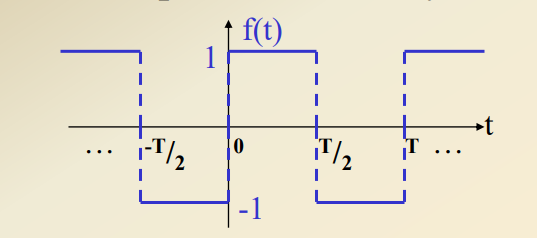
\includegraphics[width=0.5\textwidth]{fourier/volpa/image2.png}
		\centering
		\caption{Ejemplo de serie de fourier}
	\end{figure}
	\[
		f\left( t \right)\{ 1 = 0\ a\ \dfrac{T}{2};\  - 1 = \frac{T}{2}\ a\ T\ \}
	\]

	\[
		C_{n} = \dfrac{1}{T}\left( \int_{0}^{\frac{T}{2}}e^{- jn\omega_{0}t}dt + \int_{\frac{T}{2}}^{T}{- e}^{- jn\omega_{0}t}dt \right)
	\]

	\[
		C_{n} = \dfrac{1}{T}\left( \frac{1}{- jn\omega_{0}}\left( e_{}^{- jn\omega_{0}t}|_{0}^{\frac{T}{2}} - e_{}^{- jn\omega_{0}t}|_{\frac{T}{2}}^{T} \right) \right)
	\]

	\[
		C_{n} = - \dfrac{1}{Tjn\omega_0} \left[\left(e^{-\frac{jn\omega_{0}T}{2}}-1\right)-\left(e^{-jn\omega_{0}T}-e^{-\frac{jn\omega_{0}T}{2}}\right)\right]
	\]


	Recordando que
	\(\omega_{0} = \dfrac{2\pi}{T}\ e^{+ j\theta} = \cos(\theta) + j\x \sen(\theta) \)
	y las identidades trigonométricas del seno y el coseno:
	\( \cos(n\pi) = (-1)^n \)

	\[
		C_{n} = - \dfrac{1}{jn2\pi}\left[\left(\left(-1\right)-1\right)-\left(1-\left(-1\right)\right)\right]
	\]

	\[
		C_{n} = - \dfrac{2}{jn2\pi}\left\lbrack ( - 1)^{n} - 1 \right\rbrack\ 
	\]
	\[
		f(t) = - \dfrac{1}{j\pi}\left\lbrack ( - 1 )^{1} - 1 \right\rbrack e^{j\omega_{0}t} - \frac{1}{j2\pi}\left\lbrack ( - 1)^{2} - 1 \right\rbrack e^{j2\omega_{0}t} - \frac{1}{j3\pi}\left\lbrack ( - 1 )^{3} - 1 \right\rbrack e^{j3\omega_{0}t} - \ldots
	\]

	\[
		\dfrac{1}{j\pi}\left\lbrack \frac{1}{(- 1)} - 1 \right\rbrack e^{- j\omega_{0}t} + \frac{1}{j2\pi}\left\lbrack \frac{1}{( - 1 )^{2}} - 1 \right\rbrack e^{- j2\omega_{0}t} + \frac{1}{j3\pi}\left\lbrack \frac{1}{( - 1 )^{3}} - 1 \right\rbrack e^{- j3\omega_{0}t} + \ldots\ 
	\]

	Dando un paso más, a la Transformada de Fourier accedemos a lo que se
	llama la \emph{composición espectral} de una señal, que son las
	amplitudes de las diferentes componentes de frecuencia (por eso cuando
	nosotros realizamos el análisis teórico de los gráficos de frecuencia,
	vemos que los intervalos en los que \(n\omega_{0}\) existe, están
	representados con una delta de Dirac).

	\begin{figure}[H]
	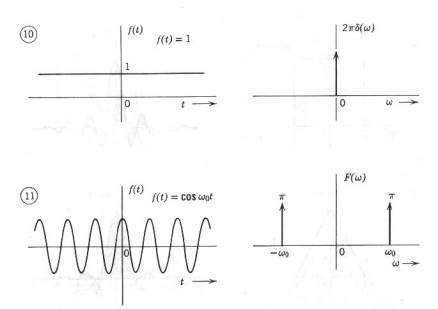
\includegraphics[width=0.5\textwidth]{fourier/volpa/image3.png}
	\centering
		\caption{Delta de Dirac}
	\end{figure}

	Yendo a un caso más concreto, si nosotros tenemos, por ejemplo, una
	señal de audio, en el análisis lo que en realidad estamos viendo es la
	composición espectral que tiene el sonido a través del aire, y lo que en
	realidad estamos viendo cuando el gráfico aumenta y reduce la amplitud
	de su señal, son deltas de Dirac imperfectas (ya que la delta de Dirac
	se utiliza para el análisis teórico) que al mismo tiempo son los
	\emph{armónicos} de mi frecuencia fundamental (los múltiplos enteros que
	vemos en la serie trigonométrica).\\
	Si después uno quisiese convertir al espectro del sonido en una señal
	del dominio del tiempo, tendría que usar a la Anti-Transformada de
	Fourier.

\subsection{Fenómeno de Gibbs}

	Vamos a analizar al fenómeno de Gibbs con la Serie Geométrica de Fourier
	del siguiente ejemplo:
\begin{figure}[H]
	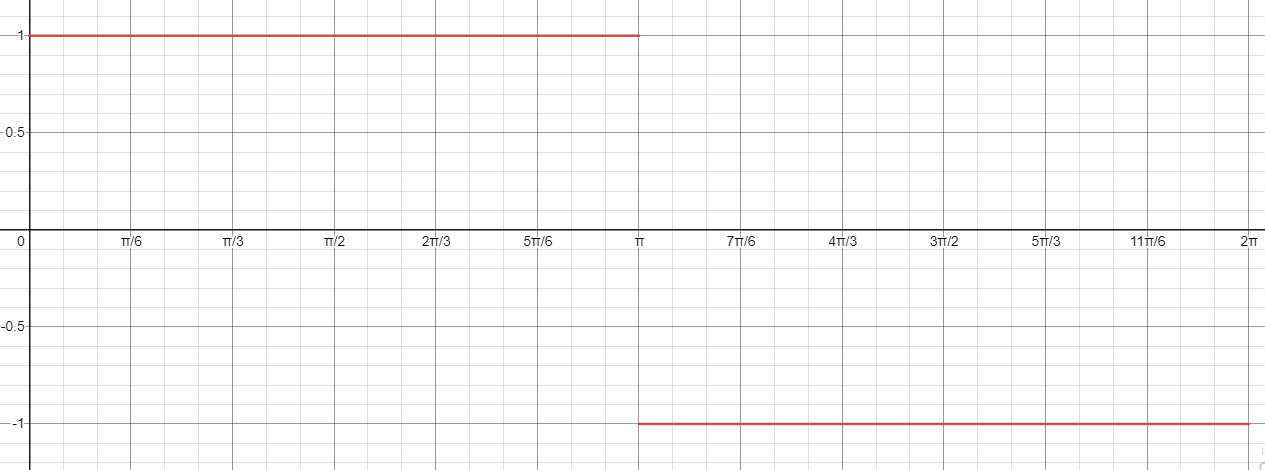
\includegraphics[width=\textwidth]{fourier/volpa/image4.png}
\end{figure}
	Tenemos que la serie trigonométrica de Fourier es la siguiente:
	\[
		f(x) = \sum_{n = 1}^{\infty} 
		\dfrac
			{4\sin((2n-1)x)}
			{(2n-1)\pi}
	\]

	Vamos a ver a los siguientes 4 casos
	\begin{enumerate}
		\item Para n= 5 --- figura número \ref{n5}
		\item Para n= 10 --- figura número \ref{n10}
		\item Para n= 25 --- figura número \ref{n25}
		\item Para n= 100 --- figura número \ref{n100}
	\end{enumerate}
	\begin{figure}[H]
		\centering
		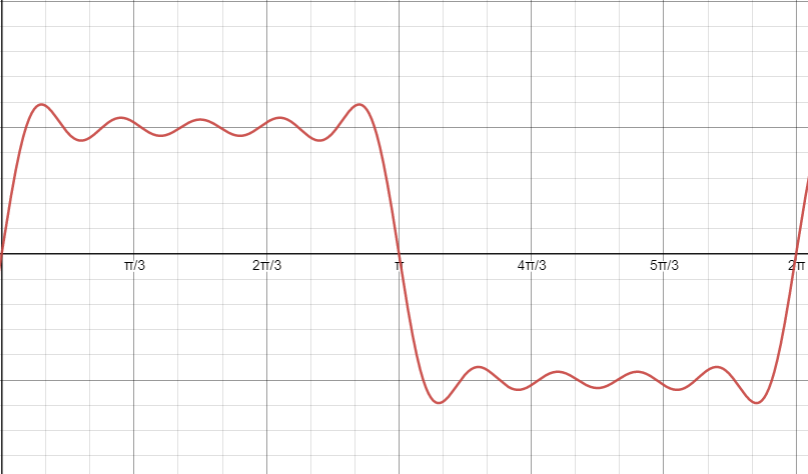
\includegraphics[width=\textwidth]{fourier/volpa/image5.png}
		\caption{Serie de Fourier para n=5}
		\label{n5}
	\end{figure}
	\begin{figure}[H]
		\centering
		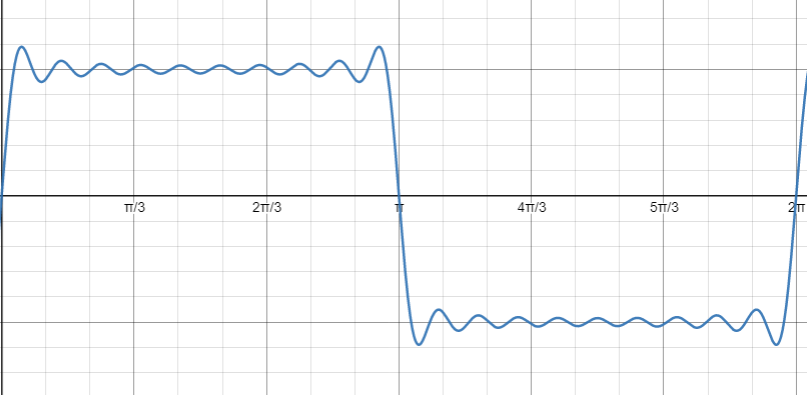
\includegraphics[width=\textwidth]{fourier/volpa/image6.png}
		\caption{Serie de Fourier para n=10}
		\label{n10}
	\end{figure}
	\begin{figure}[H]
		\centering
		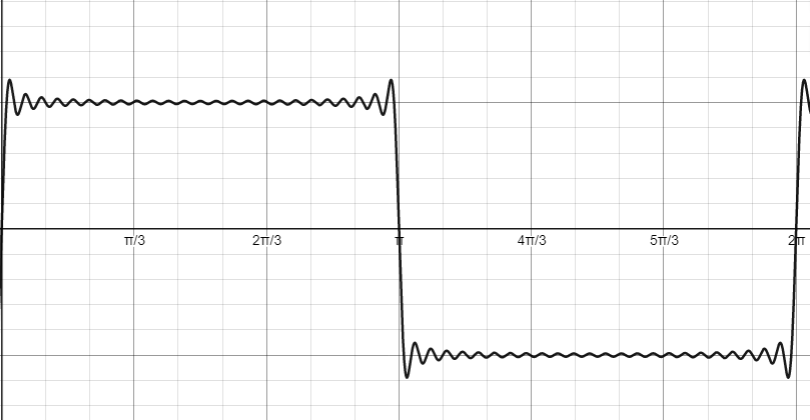
\includegraphics[width=\textwidth]{fourier/volpa/image7.png}
		\caption{Serie de Fourier para n=25}
		\label{n25}
	\end{figure}
	\begin{figure}[H]
		\centering
		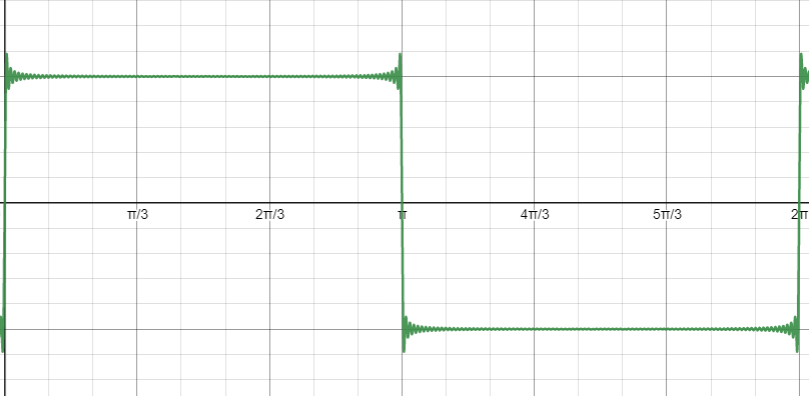
\includegraphics[width=\textwidth]{fourier/volpa/image8.png}
		\caption{Serie de Fourier para n=100}
		\label{n100}
	\end{figure}
	Lo que vemos que sucede con las aproximaciones es que cuantos más
	términos hay, naturalmente, más se acerca a nuestra función original,
	excepto por una parte, y es cuando la función está llegando a su
	discontinuidad.

	Vemos que cuando la aproximación se acerca más y más a
	dicho punto (conforme aumentan los armónicos) surge un
	\emph{sobrepasamiento} (del inglés Overshoot) que son esa especie de
	``picotazos'', los cuales no varían en su amplitud sin importar la
	cantidad de armónicos que uno vaya sumando a la serie.

	\emph{Este sobrepasamiento es aquel conocido como fenómeno de Gibbs.}

\end{document}
